\documentclass{article}

\usepackage{explorations}
\lesson{1.2.0.2 --- Money Stacks}
\module{Module 1}
\course{Explorations 1}

\begin{document}
\subsection*{Dollar Bills}

\begin{notes}Instructor: give students one or two simple examples computing volume of a rectangular
box. Note that they do not need to know or understand the volume formula yet. The goal
is to give them background information to do the activity.

Give each group of students a one-dollar bill. \end{notes}
\begin{enumerate}
\item  Give a rough estimate for the volume of the bill. Describe your thought process.

  \vspace{2in}
  
\begin{notes}
  Answer is varied. One suggestion: fold the bill several times to create a thickness.
Estimate the dimensions of the ``box''.
\end{notes}
\student{\vspace{1in}}
\begin{notes}
  Background: one dollar bills have width of 2.61 inches, length of 6.14 inches, and thickness
of 0.0043 inch. Note to instructor: do not give students these measures until they finish
the first activity above.
\end{notes}
\item\student{Your instructor will give you the measurements of a dollar bill. Write down the information here.

    \vspace{0.25in}}

  Find the height of a stack of 500 brand new one-dollar bills. Mark the height of the stack on the ruler.
  \begin{figure*}[h!]
    \centering
    \begin{minipage}{0.25\linewidth}
      
\includegraphics[width=0.9\textwidth]{stack.png}
    \end{minipage}
    \begin{minipage}{0.7\linewidth}
      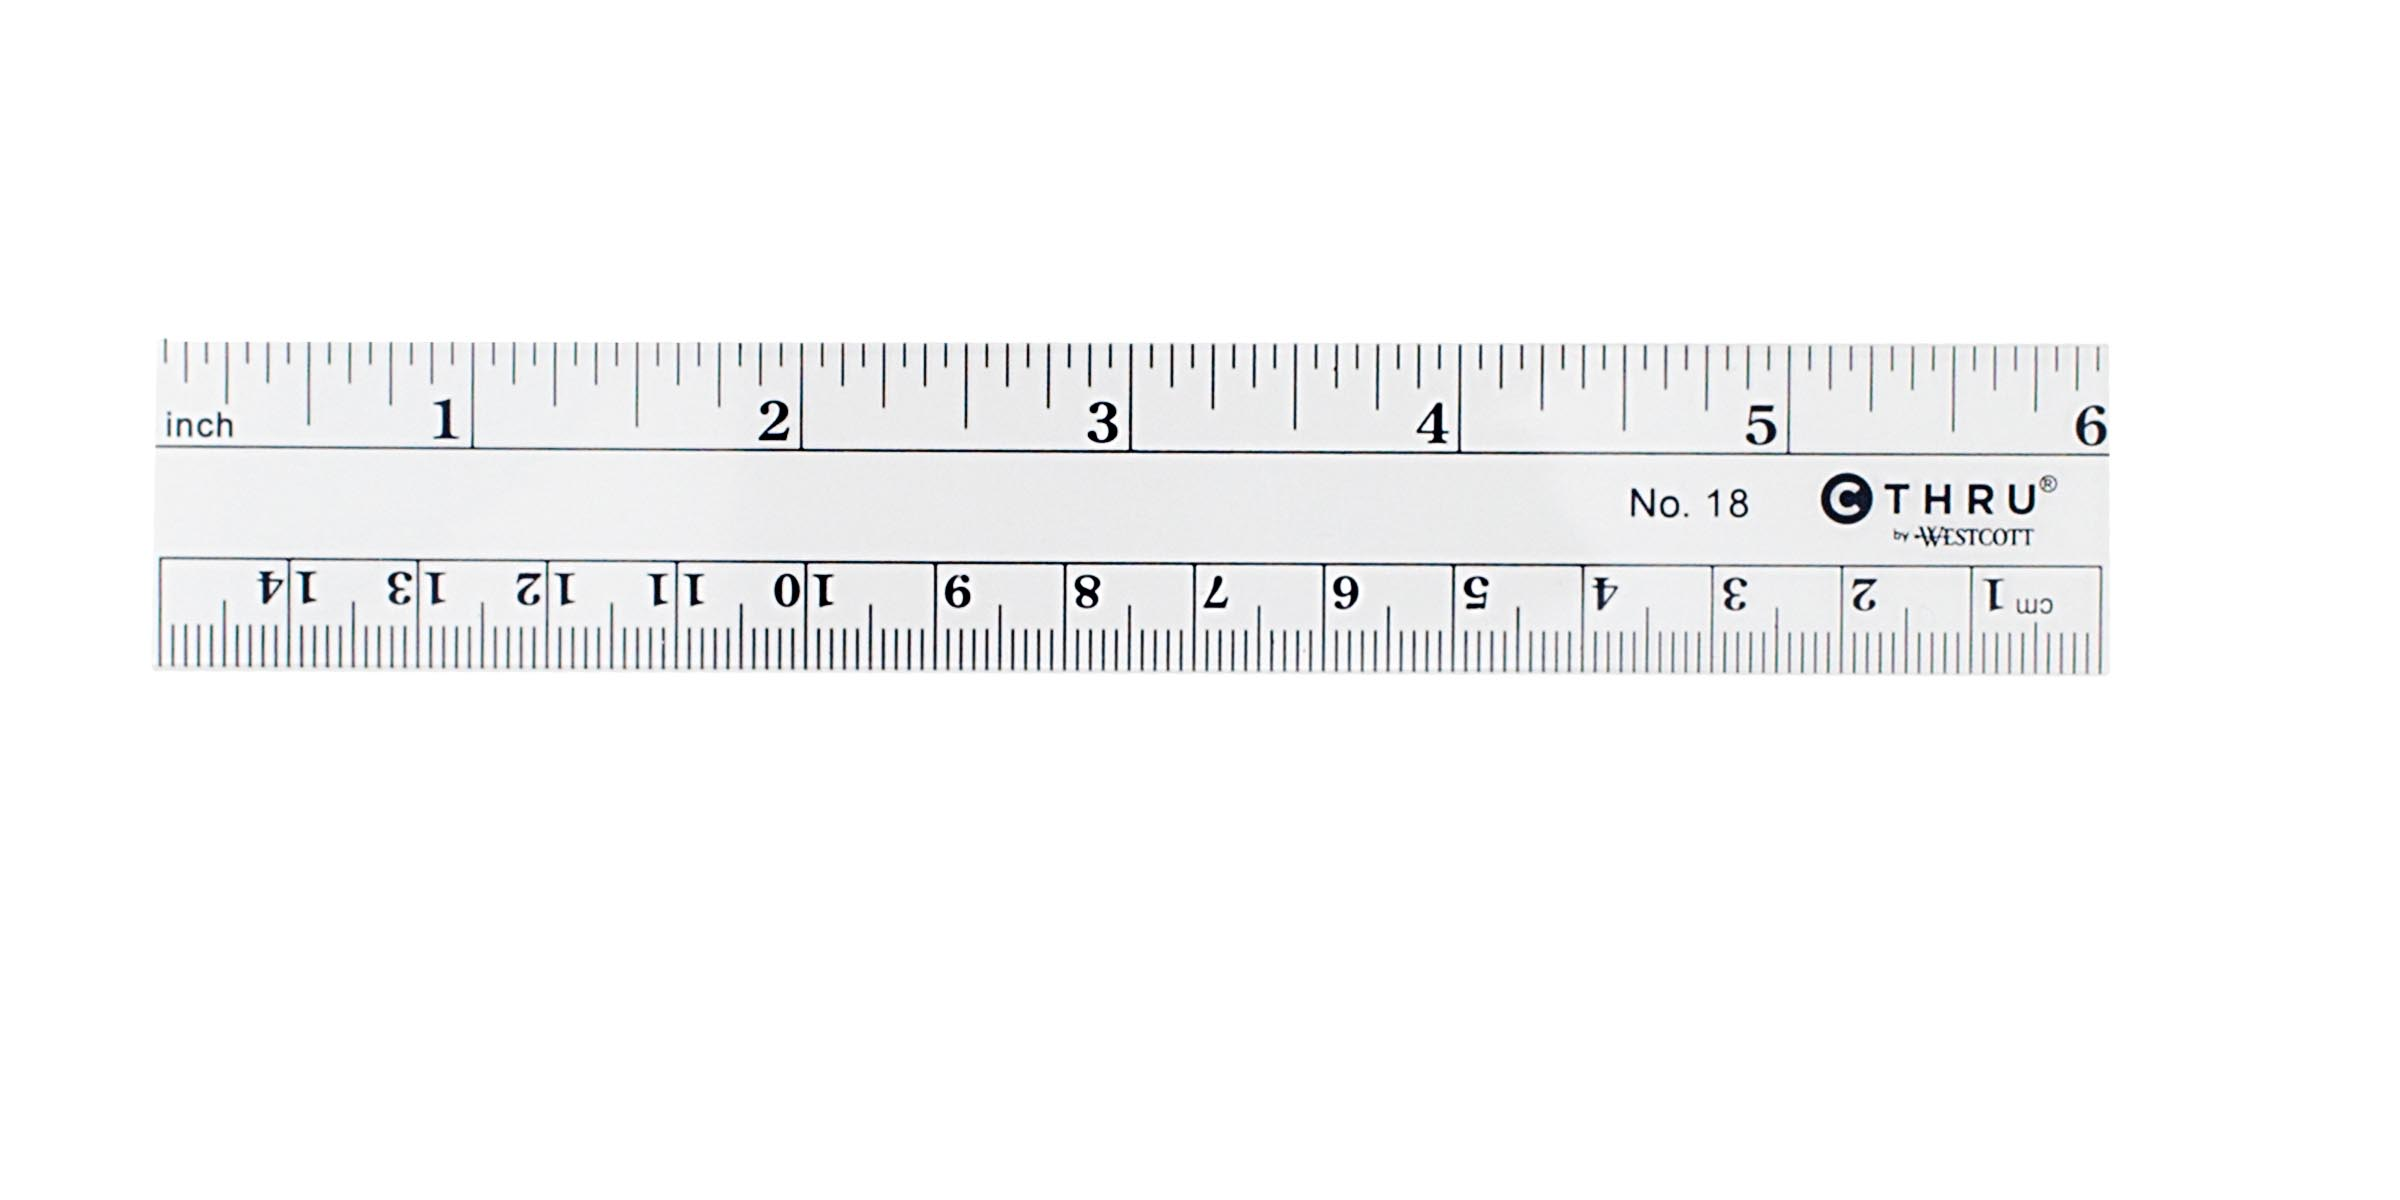
\includegraphics[width=0.9\textwidth]{ruler.png}
    \end{minipage}
  \end{figure*}
  \begin{notes}
    Answer \(500 \times 0.0043 = 2.15\) inches. If students give reasonable and logical estimations, that is OK, too.
  \end{notes}
  \student{\vspace{1in} \\ \clearpage}
\item How about a stack of 5000 brand new bills.

  \vspace{1.5in}
  
\item Which would you choose: a \SI{2}{\in} stack of one dollar bills or 5 one-hundred dollar bills? Why?

  \vspace{1.5in}
  
\item Give an estimate of the number of bills needed to be as long as the whiteboard when laid out lengthwise end-to-end.

  \vspace{1.5in}
  
\item Measure the length of the whiteboard. Use this to compute the number of bills needed. How close was your estimate?
\end{enumerate}

\mynewpage

\hfill Name:\underline{\hspace{1.5in}}
\section*{Homework}
The length of a briefcase is 17.6 inches, the width is 12.9 inches and
the height is 5.9 inches.  Feel free to use your calculators in this
activity.The bottom of the briefcase has the shape of the following
rectangle:

\begin{figure*}[h!]
  \centering
  \begin{minipage}{0.5\textwidth}
    \resizebox{0.9\textwidth}{!}{
      \begin{tikzpicture}
        \draw[thick] (0,0) rectangle (17.6,12.9);
        \node[anchor = west] at (17.6,6.5) {\Huge \SI{12.9}{\in}};
        \node[anchor = north] at (8.8,-0.1) {\Huge \SI{17.6}{\in}};
      \end{tikzpicture}
    }
  \end{minipage}
  \begin{minipage}{0.4\textwidth}
    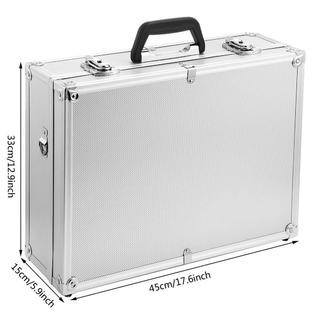
\includegraphics[width=0.9\textwidth]{briefcase.png} 
  \end{minipage}
\end{figure*}

\begin{enumerate}
\item How many dollar bills would you need to cover as much of the
  bottom of the briefcase as possible? The dollar bills can’t
  overlap. Recall that the dimensions of a dollar bill are 2.61 inches
  by 6.14 inches by 0.0043 inches Draw the dollar bills in the
  rectangle above as best you can to scale. Show any computations you
  used here.

  \vfill
  
\item Can you find a way to use more dollar bills to cover the bottom
  if the bills don’t overlap?  (Hint: Is there another way to arrange
  the bills on the bottom?)

  \vfill

  \clearpage
  
\item You decide to stack dollar bills on each of your dollar bills
  you drew in the bottom of the briefcases? How many dollar bills will
  fit in each of your stacks?

  \vfill
  
\item How much money fits in the briefcase? Use your drawing, and
  assume you stack the bills as high as possible to fit in the
  briefcase.

  \vfill
  
\item If instead of one \$1 bills you had \$100 bills, how much money would fit in the briefcase?

  \vfill
  
\end{enumerate}
\end{document}

%%% Local Variables:
%%% mode: latex
%%% TeX-master: t
%%% End:
